\chapter{Теоретические основы формирования изображений в радиолокационном и оптическом диапазонах}
\label{sec:Chapter1} \index{Chapter1}

Данная глава посвящена рассмотрению физических основ получения изображений дистанционного зондирования Земли в двух принципиально различных диапазонах электромагнитного спектра: радиолокационном и оптическом.
Понимание механизмов формирования данных, их геометрических и радиометрических особенностей является критически важным для корректной постановки задачи трансфера изображений.
Без анализа природы спекл-шума, особенностей обратного рассеяния SAR и спектральных характеристик отражения в оптическом диапазоне невозможно спроектировать эффективную архитектуру генеративной нейронной сети и правильно интерпретировать получаемые результаты.

\section{Физические принципы радиолокационной съёмки с синтезированной апертурой (РСА/SAR)}
Радиолокация с синтезированной апертурой (РСА, англ. Synthetic Aperture Radar -- SAR) относится к классу активных систем дистанционного зондирования.
В отличие от пассивных оптических сенсоров, регистрирующих отраженное солнечное излучение, радар сам облучает земную поверхность когерентным электромагнитным импульсом в микроволновом диапазоне (длины волн от 1 мм до 1 м) и регистрирует отраженный обратный сигнал.

Ключевой принцип работы SAR заключается в использовании движения носителя (самолета или спутника) для моделирования антенны, размер которой значительно превышает физический размер реальной антенны.
При движении платформы радар многократно излучает импульсы и принимает отклик от одной и той же области поверхности под разными углами.
Последующая когерентная обработка этих сигналов позволяет сформировать изображение с высоким пространственным разрешением в азимутальном направлении (вдоль траектории полета), которое теоретически не зависит от дальности до цели и не ухудшается с высотой орбиты.

Разрешение по наклонной дальности $R_r$ в SAR определяется шириной полосы пропускания зондирующего импульса $B$:
$$
R_r=\frac{c}{2B},
$$
где $c$ -- скорость света.

Основной измеряемой SAR-системой величиной является удельная эффективная площадь рассеяния (УЭПР, англ. Radar Cross Section -- RCS) или коэффициент обратного рассеяния $\sigma^0$.
Значение $\sigma^0$ зависит от диэлектрической проницаемости и влажности подстилающей поверхности, ее шероховатости, а также от угла падения луча и поляризации сигнала (VV, HH, VH, HV).
Это свойство делает SAR-снимки уникальным источником информации о структурных свойствах объектов и влажности почв, которые не видны в оптике.

\subsection{Специфические особенности РЛИ:}
\begin{enumerate}[label*=\arabic*.]
    \item \textbf{Спекл-шум}: Вследствие когерентности излучения, обратный сигнал от множества элементарных отражателей в пределах одного элемента разрешения интерферирует, создавая зернистую структуру -- спекл. Этот шум носит мультипликативный характер и существенно осложняет визуальную интерпретацию и применение классических алгоритмов компьютерного зрения, основанных на анализе градиентов яркости.
    \item \textbf{Геометрические искажения}: РЛИ часто формируется в наклонной дальности, из-за чего происходят следующие искажения:
    \begin{enumerate}[label*=\arabic*.]
        \item Радарные тени (англ. \textit{Shadowing}) -- зоны за высокими объектами (горами, зданиями), куда не попадает радиоизлучение. На снимке они выглядят как абсолютно черные пятна без полезной информации.
        \item Сокращение склонов (англ. \textit{Foreshortening}) -- склоны рельефа, обращенные к радиолокатору, кажутся короче, чем они есть на самом деле. Это происходит потому, что вершина и подножие горы находятся на близком расстоянии по наклонной дальности.
        \item Наложение склонов (англ. \textit{Layover}) -- крайний случай сокращения склонов, когда вершина горы находится ближе к радару, чем ее подножие. На изображении вершина «падает» по направлению к датчику и накладывается на подножие.
        \item Искажение масштаба (англ. \textit{Scale Distortion}) -- масштаб РЛИ непостоянен по ширине кадра. В зоне ближе к траектории полета сжатие изображения сильнее, чем в дальней.
    \end{enumerate}
    \item \textbf{Независимость от освещенности и погодных условий}: Способность получать снимки в любое время суток и сквозь атмосферные препятствия, такие как облака, является ключевым преимуществом РЛС, однако результатом является монохромное изображение, лишенное естественного цвета, что затрудняет восприятие человеком.
\end{enumerate}

\section{Особенности мультиспектральных оптических данных ДЗЗ}
Оптические системы дистанционного зондирования (например, спутники серий Landsat, Sentinel-2, WorldView или съемка с самолета) получают цифровые снимки, зафиксированные одновременно в нескольких узких диапазонах электромагнитного спектра (обычно от 3 до 15 каналов).
В отличие от радиолокационных данных, которые регистрируют отраженную радиоволну, мультиспектральные датчики пассивно фиксируют отраженный от земной поверхности и прошедший через атмосферу солнечный свет в видимом, ближнем и коротковолновом инфракрасном диапазонах.

Мультиспектральность обозначает одновременное получение изображений в нескольких спектральных каналах.
Каждый пиксель такого снимка представляет собой вектор значений энергетической яркости (или коэффициента спектральной яркости) $L(\lambda)$.

Оптические данные обладают следующими характеристиками, обратными РЛИ:
\begin{enumerate}[label*=\arabic*.]
    \item \textbf{Высокая цветовая и текстурная информативность}: Видимый диапазон позволяет получать изображения в естественных цветах, естественных для человеческого восприятия. Это критически важно для визуального анализа.
    \item \textbf{Зависимость от атмосферы}: Наличие атмосферных искажений, например, облаков, дымки, аэрозолей и тени от облаков блокирует или искажает полезный сигнал отраженный от земной поверхности. Это приводит к пробелам в данных и делает оперативный мониторинг в некоторых регионах крайне затруднительным.
    \item \textbf{Сезонная и суточная изменчивость}: Яркость оптического изображения сильно зависит от высоты солнца и фенологического состояния растительности. Это усложняет сопоставление снимков, сделанных в разное время во временные ряды.
\end{enumerate}

\subsection{Уравнение переноса излучения (упрощенная модель)}
Сигнал, регистрируемый сенсором $L_\text{сенсор}$, может быть представлен как:
$$
L_\text{сенсор} = L_\text{отраж} \cdot T_\text{атм} + L_\text{рассеян},
$$
где $L_\text{отраж}$ -- отраженное поверхностью излучение, 
$T_\text{атм}$ -- пропускание атмосферы, 
$L_\text{рассеян}$ -- атмосферная дымка.

Это уравнение показывает, что оптический пиксель является интегральной характеристикой как свойств поверхности, так и состояния атмосферы на момент съемки.

\section{Сравнительный анализ доменов SAR и Optical}
Сопоставление радиолокационного и оптического доменов выявляет фундаментальный семантический разрыв, который является главным препятствием для совместного использования данных и мотивирует задачу трансфера стиля изображений.
В таблице \ref{tab:sar_vs_optical} приведено сравнение ключевых свойств двух типов данных.

\begin{table}[!ht]
\centering
\caption{Сравнительная характеристика радиолокационных (SAR) и оптических данных дистанционного зондирования}
\label{tab:sar_vs_optical}
\begin{tabular}{|p{4cm}|p{6cm}|p{5cm}|}
\hline
\textbf{Характеристика} & \textbf{Радиолокационные данные (SAR / Sentinel-1)} & \textbf{Оптические данные (Sentinel-2 / Landsat)} \\
\hline
Тип сенсора & Активный & Пассивный \\
\hline
Физика сигнала & Обратное рассеяние радарного импульса \( \sigma^0 \) & Отражение солнечного света \( \rho \) \\
\hline
Зависимость от погоды & Всепогодность (облака прозрачны) & Критическая, требуется безоблачность \\
\hline
Время съемки & Круглосуточно & Только дневное время \\
\hline
Цветовая информация & Отсутствует (монохром, псевдоцвет) & Присутствует (RGB, NIR) \\
\hline
Шум & Мультипликативный спекл-шум & Аддитивный гауссов шум \\
\hline
Чувствительность к геометрии & Чувствительность к шероховатости и диэлектрической проницаемости & Чувствительность к затенению рельефа \\
\hline
Семантическая интерпретация & Сложна, требует насмотренности и опыта & Интуитивно понятна, естественна для восприятия \\
\hline
\end{tabular}
\end{table}

Проблема семантического разрыва заключается в том, что один и тот же физический объект имеет принципиально разное представление в двух доменах.

\paragraph{Водные поверхности}
В оптике вода выглядит темной (поглощение света). На РЛИ на гладкой воде при малых углах падения сигнал практически отсутствует (темный тон), однако при наличии ветрового волнения обратное рассеяние резко возрастает (светлый тон).

\begin{figure}[!ht]
    \centering
    \begin{subfigure}[t]{0.4\textwidth}
        \centering
        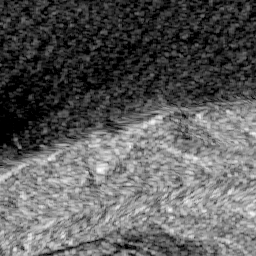
\includegraphics[width=\textwidth]{./images/sen12/ROIs1158_spring_s1_0_p19.png}
        \caption{Радиолокационное изображение (Sentinel-1, VV-поляризация)}
        \label{subfig:sar_example_water}
    \end{subfigure}
    \hspace{0.5cm}
    \begin{subfigure}[t]{0.4\textwidth}
        \centering
        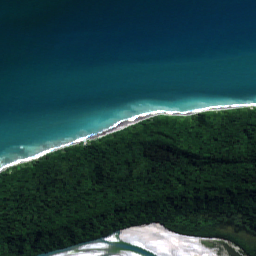
\includegraphics[width=\textwidth]{./images/sen12/ROIs1158_spring_s2_0_p19.png}
        \caption{Оптическое RGB-изображение (Sentinel-2)}
        \label{subfig:opt_example_water}
    \end{subfigure}
    \caption{Сравнение представления одного и того же участка земной поверхности (водоем) (SEN1-2~\cite{schmitt2018sen1}, ID: ROIs1158\_spring\_s\{1,2\}\_0\_p19).}
    \label{fig:sar_vs_opt_water}
\end{figure}

\paragraph{Городская застройка}
В оптике -- сложная мозаика цветов крыш и дорог.
На РЛИ -- области интенсивного рассеяния из-за эффекта двугранного уголка (уголковый отражатель), приводящего к появлению очень ярких пикселей (доминирование лейовера).

\begin{figure}[!ht]
    \centering
    \begin{subfigure}[t]{0.4\textwidth}
        \centering
        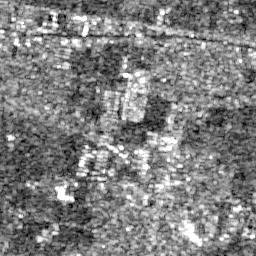
\includegraphics[width=\textwidth]{./images/sen12/ROIs1158_spring_s1_18_p42.png}
        \caption{Радиолокационное изображение (Sentinel-1, VV-поляризация)}
        \label{subfig:sar_example_urban}
    \end{subfigure}
    \hspace{0.5cm}
    \begin{subfigure}[t]{0.4\textwidth}
        \centering
        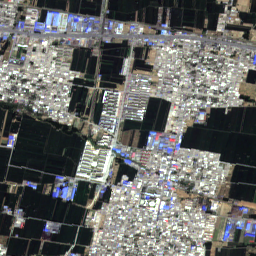
\includegraphics[width=\textwidth]{./images/sen12/ROIs1158_spring_s2_18_p42.png}
        \caption{Оптическое RGB-изображение (Sentinel-2)}
        \label{subfig:opt_example_urban}
    \end{subfigure}
    \caption{Сравнение представления одного и того же участка земной поверхности (городская застройка)\\(SEN1-2~\cite{schmitt2018sen1}, ID: ROIs1158\_spring\_s\{1,2\}\_18\_p42).}
    \label{fig:sar_vs_opt_urban}
\end{figure}

\paragraph{Растительность}
В оптике растительность идентифицируется по спектральному профилю (пик в NIR).
На РЛИ растительность характеризуется объемным рассеянием, зависящим от влажности биомассы и структуры полога (кросс-поляризация VH/HV).

\begin{figure}[!ht]
    \centering
    \begin{subfigure}[t]{0.4\textwidth}
        \centering
        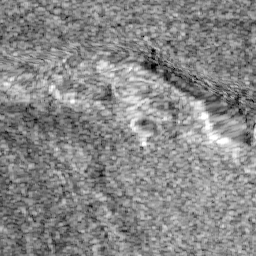
\includegraphics[width=\textwidth]{./images/sen12/ROIs1158_spring_s1_0_p22.png}
        \caption{Радиолокационное изображение (Sentinel-1, VV-поляризация)}
        \label{subfig:sar_example_grass}
    \end{subfigure}
    \hspace{0.5cm}
    \begin{subfigure}[t]{0.4\textwidth}
        \centering
        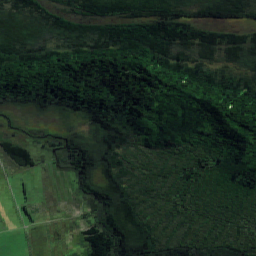
\includegraphics[width=\textwidth]{./images/sen12/ROIs1158_spring_s2_0_p22.png}
        \caption{Оптическое RGB-изображение (Sentinel-2)}
        \label{subfig:opt_example_grass}
    \end{subfigure}
    \caption{Сравнение представления одного и того же участка земной поверхности (растительность)\\(SEN1-2~\cite{schmitt2018sen1}, ID: ROIs1158\_spring\_s\{1,2\}\_0\_p22).}
    \label{fig:sar_vs_opt_grass}
\end{figure}

\paragraph{Горные и лишенные растительности участки} 
В оптике горные породы и почвы характеризуются оттенками серого и коричневого.
На РЛИ из-за пересеченного рельефа доминируют геометрические искажения: яркий форшотенинг на склонах, обращенных к радару, и глубокие радиолокационные тени на обратных склонах.

\begin{figure}[!ht]
    \centering
    \begin{subfigure}[t]{0.4\textwidth}
        \centering
        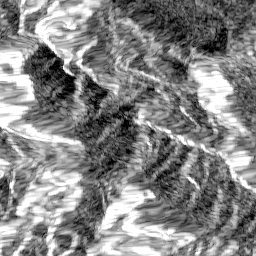
\includegraphics[width=\textwidth]{./images/sen12/ROIs1158_spring_s1_9_p155.png}
        \caption{Радиолокационное изображение (Sentinel-1, VV-поляризация)}
        \label{subfig:sar_example_mountain}
    \end{subfigure}
    \hspace{0.5cm}
    \begin{subfigure}[t]{0.4\textwidth}
        \centering
        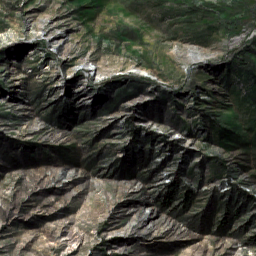
\includegraphics[width=\textwidth]{./images/sen12/ROIs1158_spring_s2_9_p155.png}
        \caption{Оптическое RGB-изображение (Sentinel-2)}
        \label{subfig:opt_example_mountain}
    \end{subfigure}
    \caption{Сравнение представления одного и того же участка земной поверхности (горная местность) (SEN1-2~\cite{schmitt2018sen1}, ID: ROIs1158\_spring\_s\{1,2\}\_9\_p155).}
    \label{fig:sar_vs_opt_mountain}
\end{figure}

Таким образом, прямое сопоставление пикселей РЛИ и оптики невозможно в силу разной физической природы формирования яркости.
Формально, если представить РЛИ как отображение функции обратного рассеяния \( \Sigma(x,y) \), а оптическое как отображение функции отражения \( \rho(\lambda, x,y) \), то не существует линейного оператора \( \mathcal{L} \) такого, что \( \mathcal{L}(\Sigma) = \rho \). 

Задача генеративного трансфера, решаемая в рамках данной работы, направлена на построение нелинейного отображения \( G: I_{SAR} \rightarrow I_{Opt} \), которое восстанавливает не точное значение коэффициента спектральной яркости (что физически невозможно без априорной информации о материале), а семантическую структуру сцены.
Иными словами, нейронная сеть \( G \) аппроксимирует условное распределение \( p(I_{Opt} | I_{SAR}) \), заменяя физический механизм когерентного рассеяния на механизм некогерентного отражения, привычный для человеческого зрения.

\section{Характеристики данных как входных сигналов для нейросетевых моделей}
Для успешного применения методов глубокого обучения к задаче трансфера SAR $\rightarrow$ Optical необходимо учитывать особенности предобработки данных, вытекающие из описанных выше физических принципов.

\begin{enumerate}[label*=\arabic*.]
    \item \textbf{Динамический диапазон и нормализация}: $\sigma^0$ (в линейном масштабе или децибелах) и коэффициентов яркости оптических снимков (отражательная способность от 0 до 1) имеют разные статистические распределения. Для подачи в нейронную сеть требуется унификация данных через приведение к диапазону [-1, 1] или [0, 1] с помощью соответствующих процедур нормализации и, в ряде случаев, логарифмирования SAR-амплитуд.
    \item \textbf{Подавление спекл-шума}: современные GAN-архитектуры, а тем более диффузионные, способны учиться игнорировать спекл или выявлять некоторые зависимости из него для последующего успешного преодоления этой особенности задачи. Также возможно применение предварительной пространственной фильтрации (например, фильтры Ли, Фроста или нелокальные средства NL-SAR, в том числе с использованием нейронных сетей), что часто улучшает сходимость обучения и снижает количество артефактов в генерируемых оптических изображениях, но требует решения отдельной задачи в нетривиальных случаях.
    \item \textbf{Геометрическое совмещение}: SAR и оптические снимки имеют разные механизмы геопривязки. Для обучения парных моделей (например, Pix2Pix) критически важно точное субпиксельное совмещение (ко-регистрация) изображений. Ошибки совмещения ведут к размытию высокочастотных деталей в результатах генерации.
    \item \textbf{Выбор поляризационных каналов}: одиночный канал (VV или VH) несет ограниченную информацию. Для более качественного трансфера цвета часто используют мультиполяризационные композиты или данные поляриметрической декомпозиции (например, Фримена-Дурдена или Клода-Поттье), которые позволяют извлечь больше физических признаков о типе рассеяния (поверхностное, объемное, двугранное).
\end{enumerate}

Однако предоставляемые наборы данных, описанные в главе~\ref{sec:Chapter2} (например, SEN1-2~\cite{schmitt2018sen1}), уже содержат предварительно обработанные и геопривязанные пары изображений, что позволяет сосредоточиться на разработке архитектуры нейронной сети и оптимизации процесса обучения, не отвлекаясь на сложные этапы предобработки, но ограничивая как разработчика сети, так и саму модель в данных для обучения.
Хотя и существует набор данных в котором представлены сырые (необработанные) SAR-изображения, их использование, помимо решения дополнительных задач, таких как подавление спекл-шума и коррекция геометрических искажений (что выходит за рамки данной работы), накладывает строгие ограничения на технические характеристики используемого оборудования и увеличивает время обучения модели и затрачиваемые на это ресурсы.
В условиях отсустствия центра обработки данных с внушительными вычислительными ресурсами, использование необработанных данных не представляется возможным. Также стоит отметить, что все существующие модели, описанные в данной работе, были обучены на предварительно обработанных и геопривязанных данных, что обеспечивает достижение поставленной цели при оптимальных затратах времени и ресурсов, а также позволяет сравнить результаты генерации и метрики, полученные в ходе обучения моделей.

\newpage